% Please do not change the document class
\documentclass{scrartcl}

% Please do not change these packages
\usepackage[hidelinks]{hyperref}
\usepackage[none]{hyphenat}
\usepackage{setspace}
\usepackage{graphicx}
\graphicspath{ {C:/Users/james/Documents/GitHub/comp140-hardware/Progress/} }
\usepackage[rightcaption]{sidecap}
\doublespace

% You may add additional packages here
\usepackage{amsmath}

% Please include a clear, concise, and descriptive title
\title{Heuristic Analysis}

% Please do not change the subtitle
\subtitle{COMP140 - Heuristic Analysis}

% Please put your student number in the author field
\author{1506530}

\begin{document}

\maketitle

\section{The Controller}
The controller is based on the Nintendo nunchuck, this was chosen for marketable reasons. As there seems to ba a lack of PC controllers for use in one hand, it seemed appropriate to use this controller as a baseline. The idea for the controller was to create a one-handed device that could be used in conjunction with a game while being able to free up the other hand. The controller was build using and Arduino UNO and a MakeyMakey kit. As the Arduino UNO does not support HID, the MakeyMakey was used as a bridge between the PC and the Arduino. Two buttons and a joystick were applied to the controller.

\section{Analysis}
The controller was build for functionality over creativity, to that end everything worked as planned. Both buttons responded to being pressed and with some tinkering the joystick recognized both the X,Y axis. The LED light that was present ensured that the user would know that a button press was being recognized. As this was done through the means of software and not hard-wired into the controller the responsiveness of the buttons was clearly seen. 
\newline Jakob Nielsen set out many heuristics to judge an items usability:
\begin{itemize}
	\item Visibility of system status
	\item Match between system and the real world
	\item User control and freedom	
	\item Consistency and standards
	\item Error prevention
	\item Recognition rather than recall
	\item Flexibility and efficiency of use
	\item Aesthetic and minimalist design
	\item Help users recognize, diagnose, and recover from errors	
	\item Help and documentation \cite{niel}
	\newline
	\newline
\end{itemize}
The two that would most benefit the controller are: 
\begin{itemize}
	\item Aesthetic and minimalist design
	\item Flexibility and efficiency of use
	\newline
		\newline
			\newline
				\newline
\end{itemize}


\subsection{Aesthetics}
\begin{figure}[h!]
	\centering
	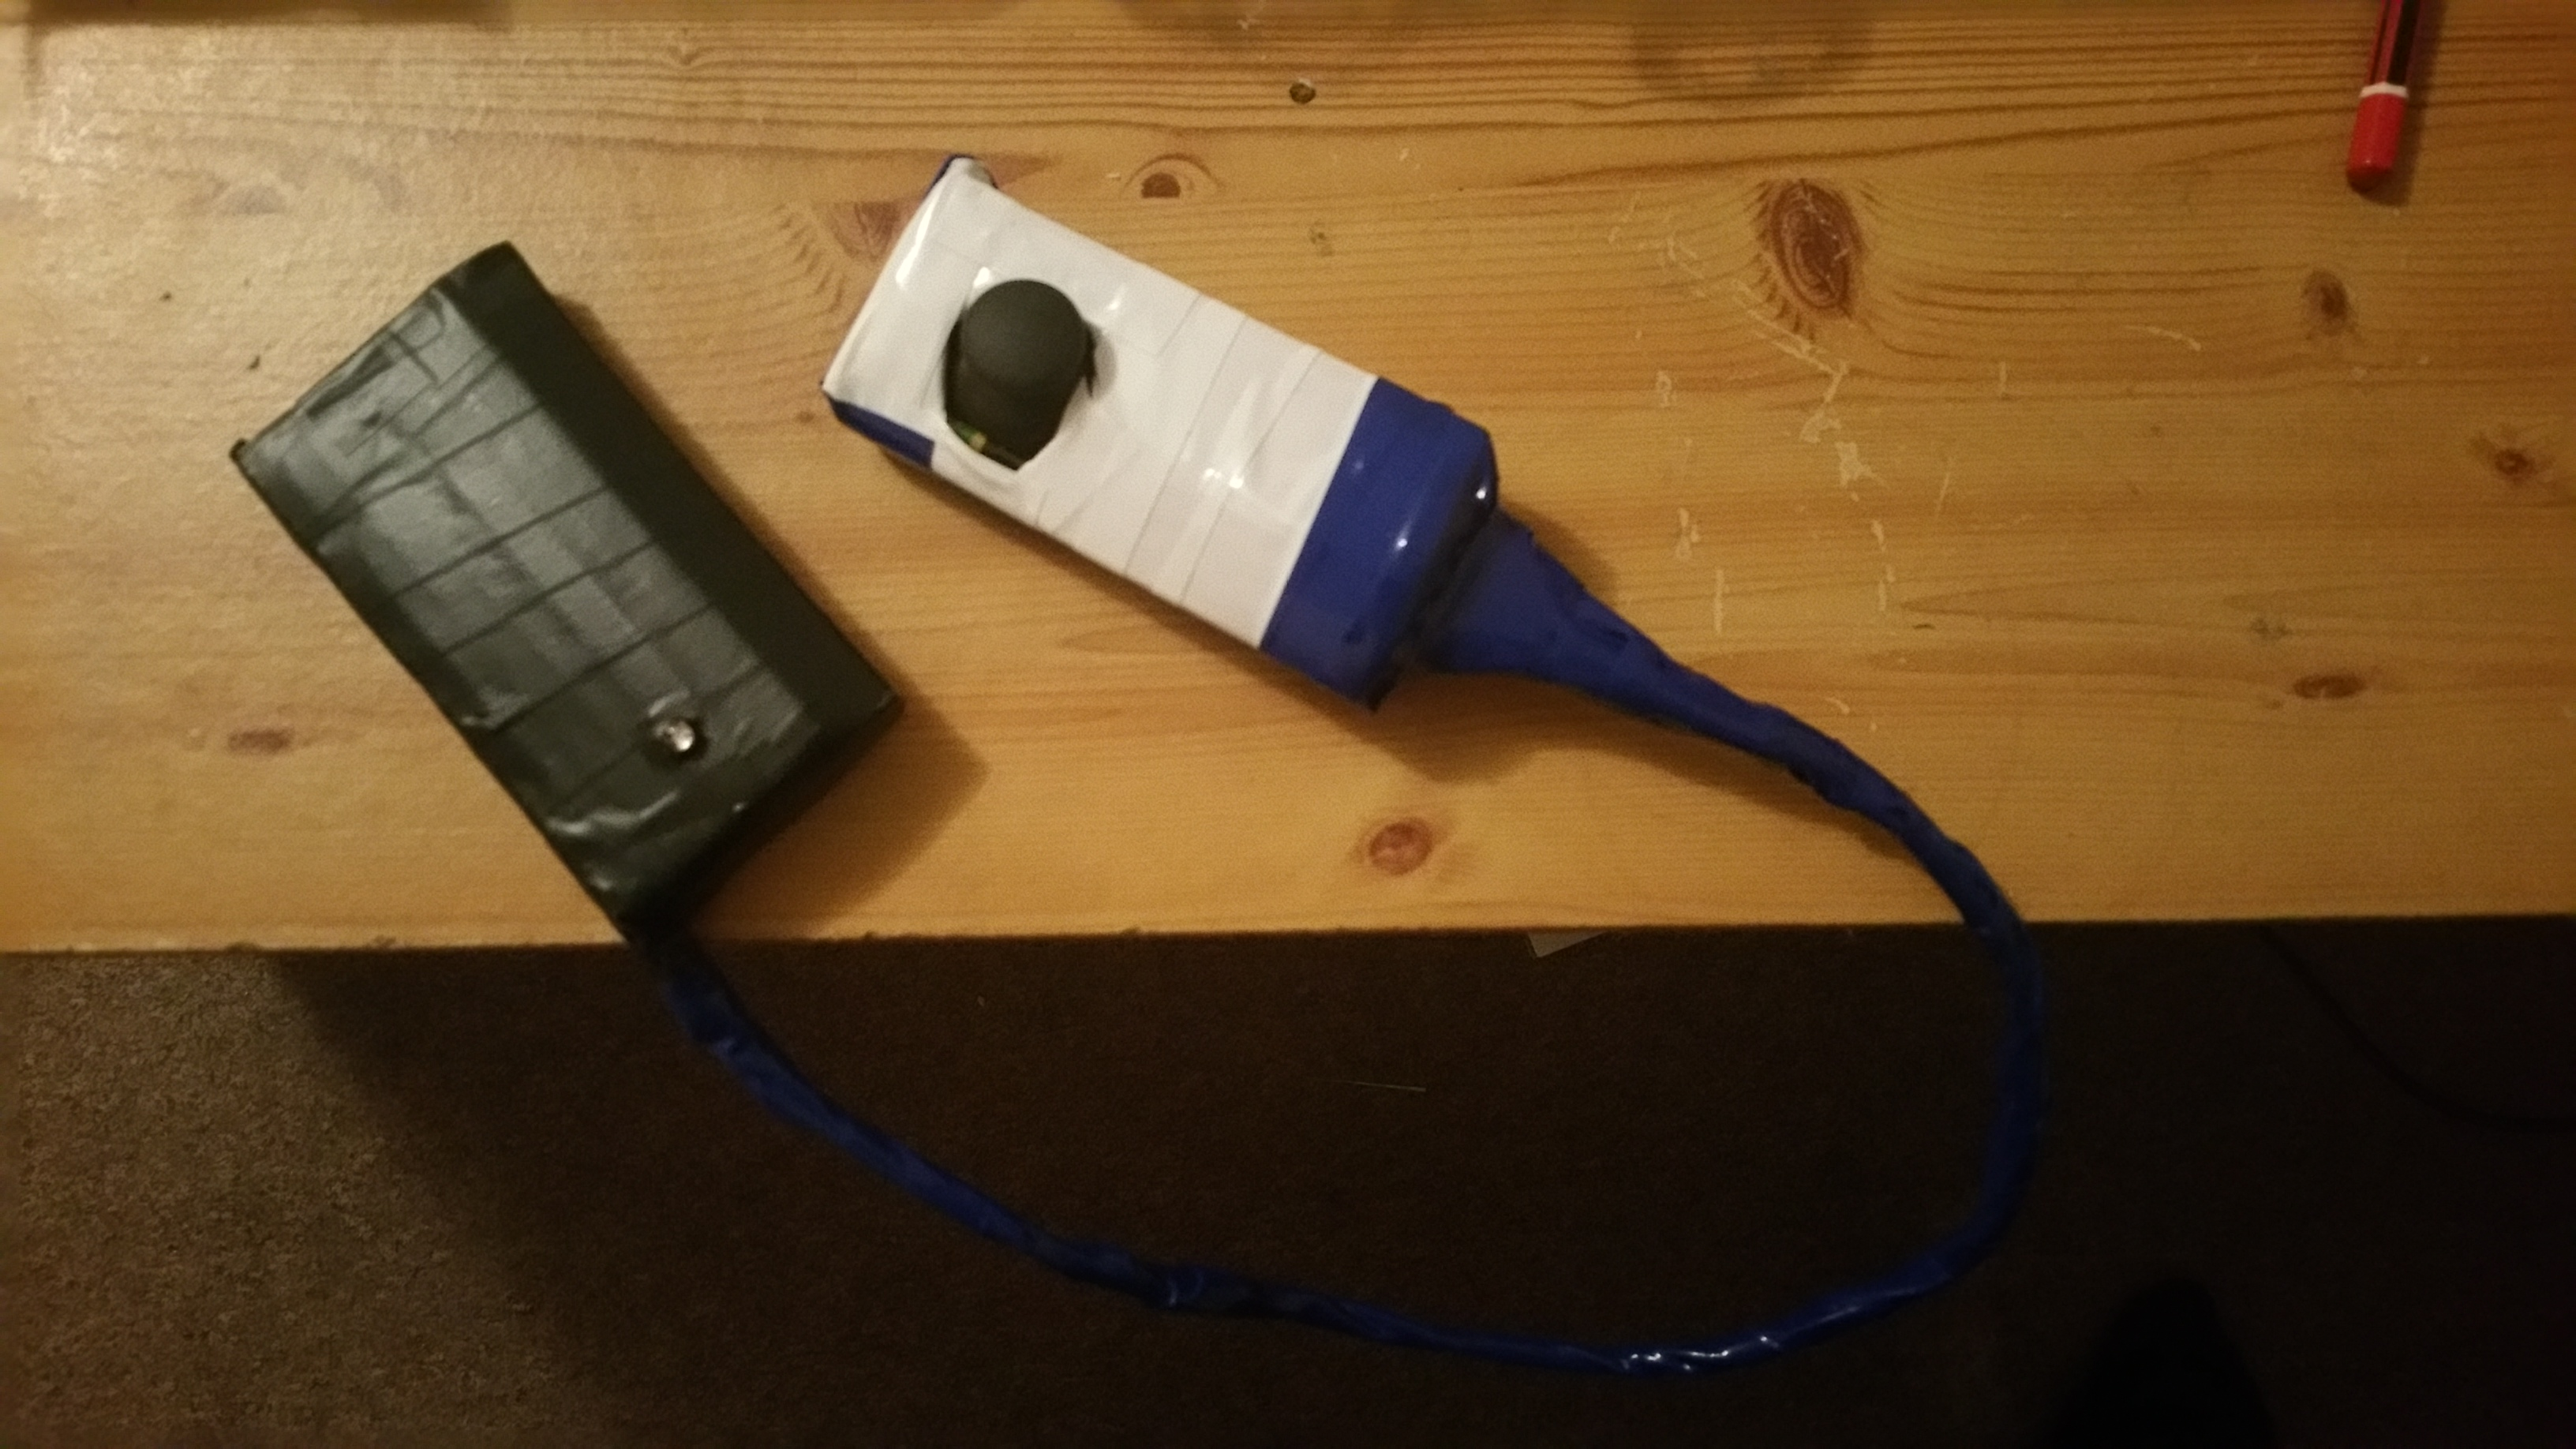
\includegraphics[width=0.7\linewidth]{Complete_Controller_06_03_2015.jpg}
	\caption{First iteration of controller}
	\label{Fig1}
\end{figure}
\begin{figure}[h]
	\centering
	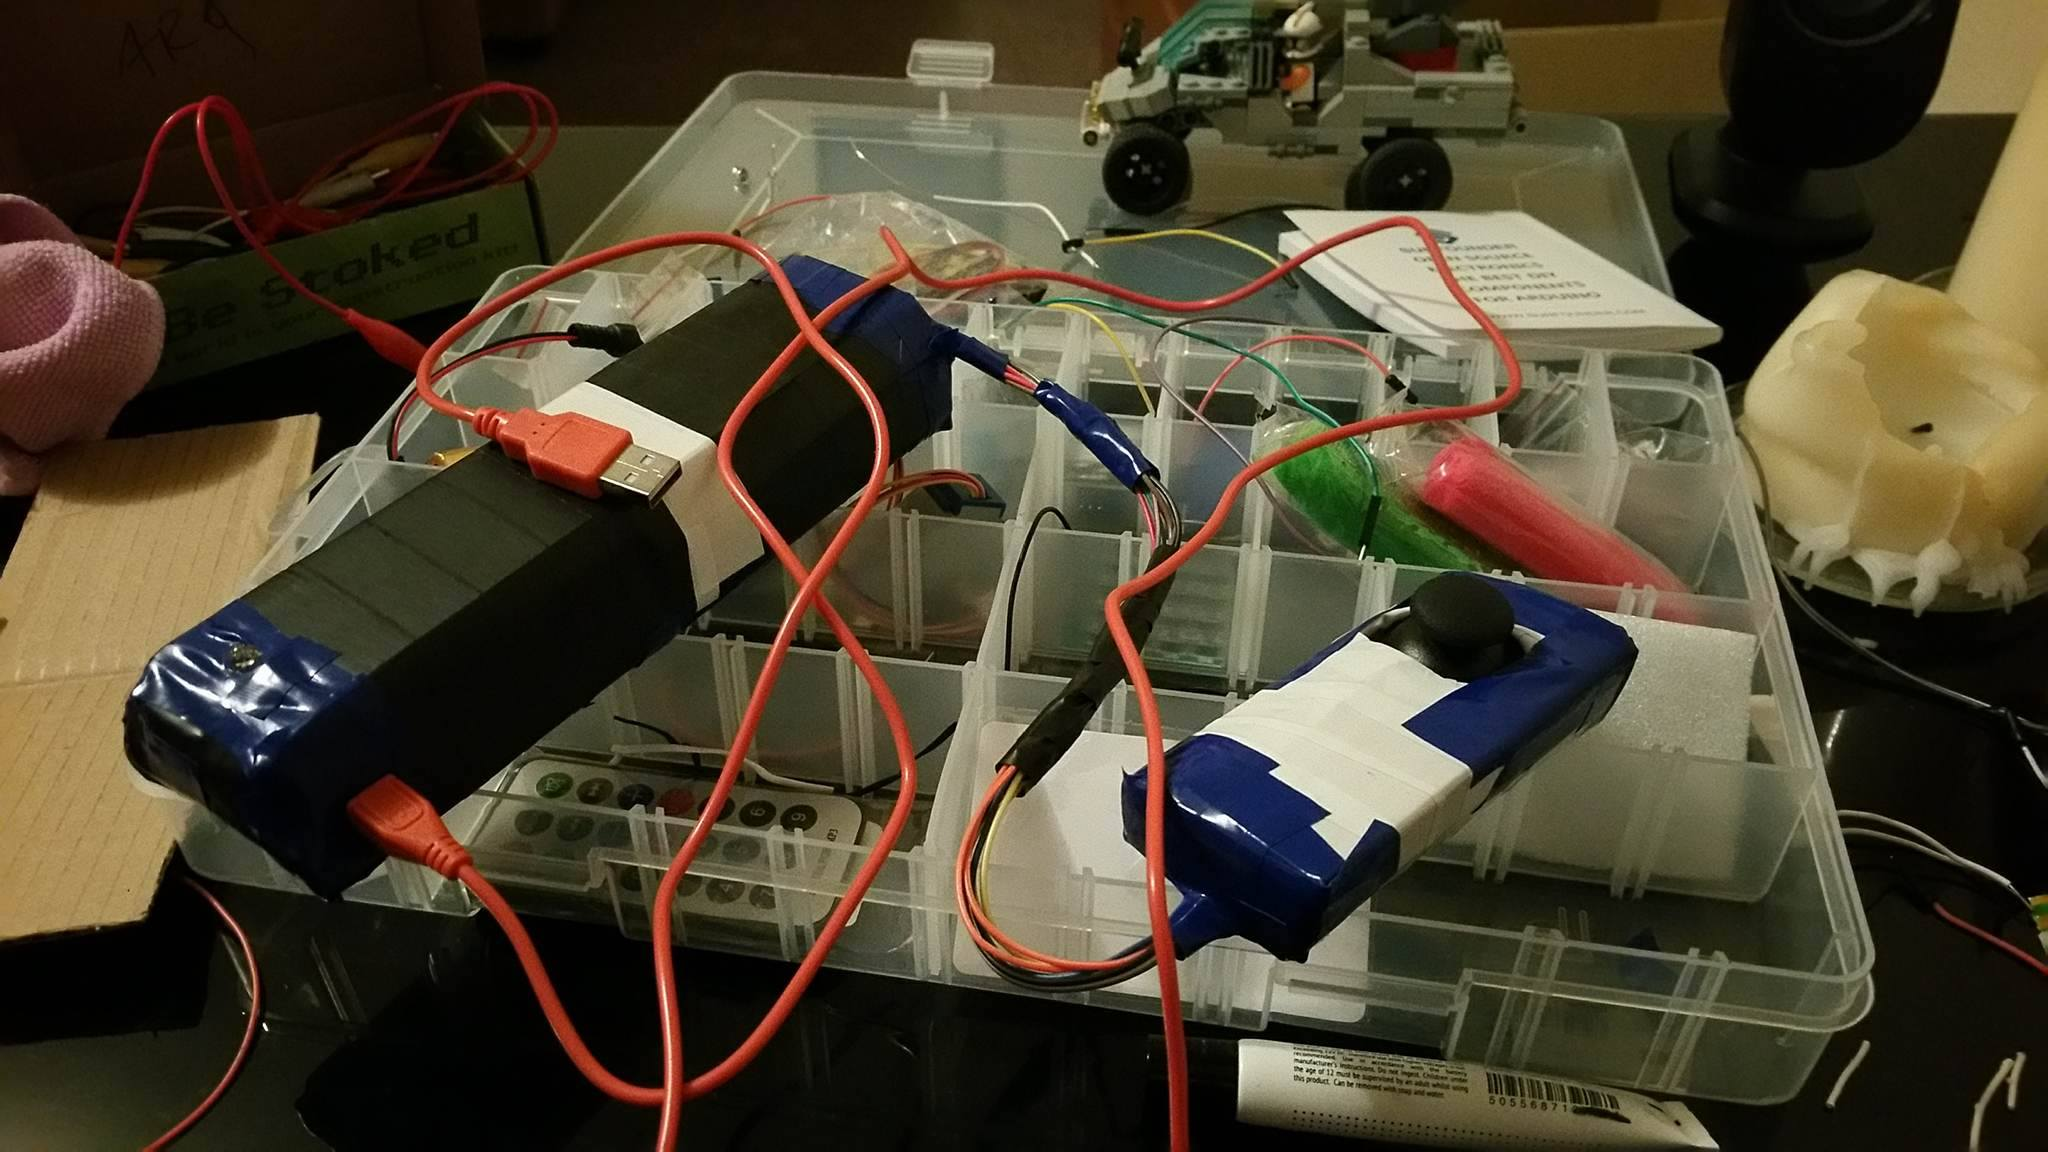
\includegraphics[width=0.7\linewidth]{Redesign_13_03_2016_Final.jpg}
	\caption{Final controller iteration}
	\label{Fig2}
\end{figure}
As can be seen in figure one and two, from an aesthetic view, the controller its self was minimalistic, although the circuit boards attached to it made for an unpleasant addition. This was due to the two board having to be connected for the PC to recognize the controller as a HID. A suggestion for improvement here would be to minimise the need for the two circuit board. To do this an Arduino Micro would have been proficient, this Arduino has a built in HID driver and would have removed the need for any wires to be present outside of the controller. This also would have allowed the removal of the large box and improved usability and aesthetics.

\begin{figure}[h]
	\centering
	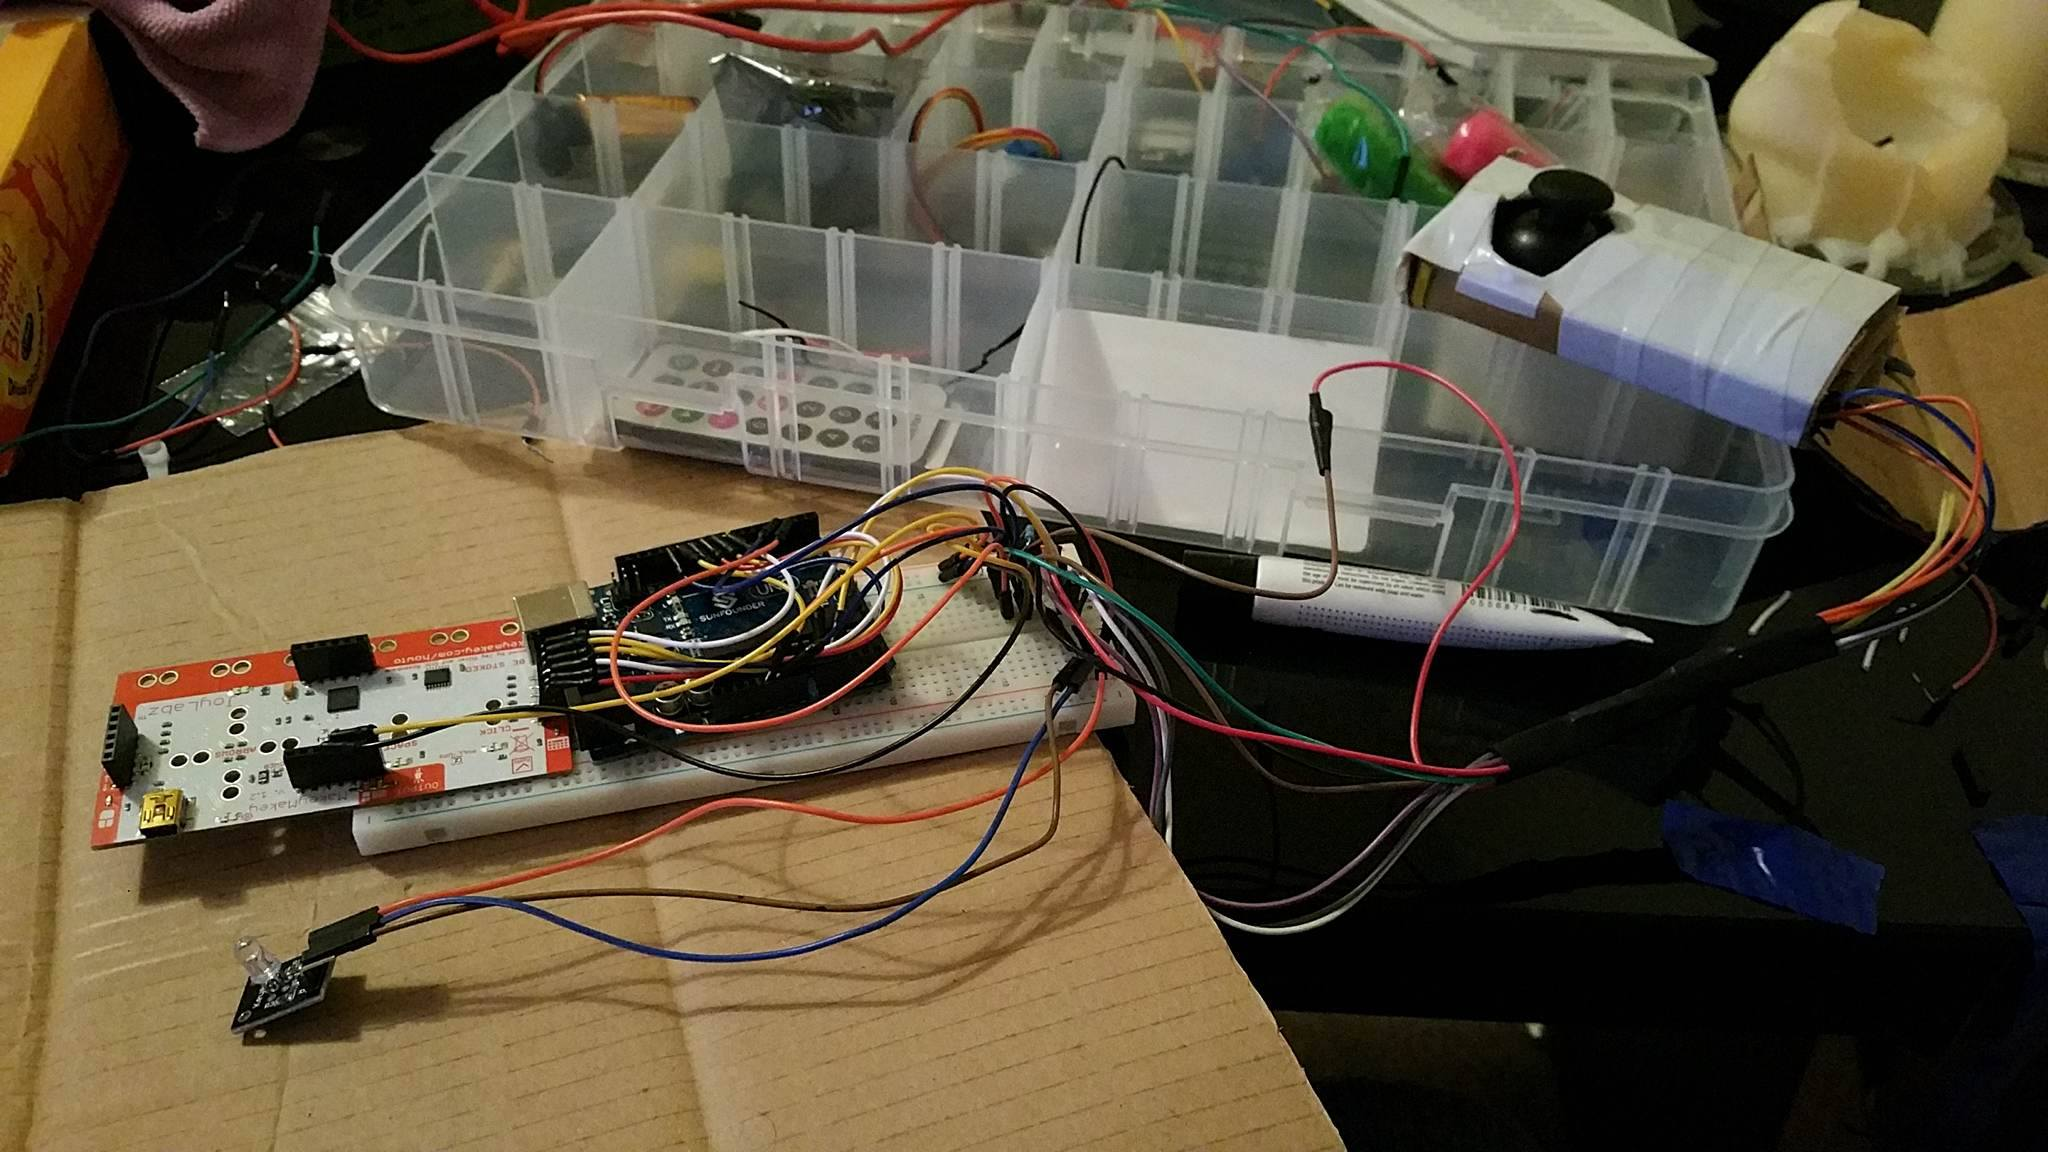
\includegraphics[width=0.7\linewidth]{Redesign_13_03_2016_Working.jpg}
	\caption{Controller Exposed To Reveal Inner Circuits}
	\label{Fig3}
\end{figure}
\subsection{Flexibility and Efficiency}
The controller was efficient in what it was planned to do, as stated at the beginning, comfortable to hold and responsive. To use, the controller was straining on the hands as the two buttons were placed at the back. Although the lack of extra buttons limited its usability, a suggested improvement would be to increase this number. Also to improve the ergonomics of the controller would be an improvement for flexibility. This would be achieved by altering the position of the buttons at the back.

\section{Final Remarks}
In retrospect it would have been advantageous to have more usability and comfort for the controller. A lot has been learnt on controller construction and it would go very differently if another was to be built.

\bibliographystyle{ieeetran}
\bibliography{COMP140_Heuristic-Analysis}

\end{document}